% KSe.tex
% $Author$ $Date$

% Predrag                   jun 20 2006
% Vaggelis                  may 20 2006

\section{\KSe}
\label{s-KS}
% Predrag                    4jul2006
% extracted from ~dasbuch/book/chapter/PDEs.tex  5jun2005 version
% Predrag                   17sep1999

% \PC{incorporate missing refs from chapter/refsPDEs.tex}

The \KS\ [KS] system\rf{ku,siv}, which
arises in the description of stability of
flame fronts, reaction-diffusion systems and many other physical settings,
is one of the simplest nonlinear PDEs that
exhibit spatiotemporally chaotic behavior.
In the formulation adopted here, the time evolution of the 
``flame front velocity'' $u=u(x,t)$ on a periodic domain
$u(x,t) = u(x+L,t)$
is given by
\beq
    u_t=(u^2)_x-u_{xx}- u_{xxxx}
    \,,\qquad   x \in [0,L]
    \,.
\ee{ks}
Here $t \geq 0$ is the time, and
$x$ is the spatial coordinate.
The subscripts $x$ and $t$ denote partial derivatives with respect to
$x$ and $t$. In what follows we use interchangeably the ``dimensionless''
system size $\tildeL$, or the periodic domain size $L= 2\pi \tildeL$,
as the system parameter.

Spatial periodic boundary condition $u(x,t)=u(x+L,t)$
makes it convenient to work in the Fourier space, 
\beq
  u(x,t)=\sum_{k=-\infty}^{+\infty} a_k (t) e^{ i k x /\tildeL }
\,,
% \label{fseries}
\ee{eq:ksexp}
%where $\tildeL=L/2\pi$. Thus, 
with the $1D$ PDE \refeq{ks}
replaced by an infinite set of 
ODEs for the Fourier coefficients:
\beq
\dot{a}_k= ( (k/\tildeL)^2 - ( k/\tildeL)^4 )\, a_k 
    + \frac{i k}{\tildeL} \sum_{m=-\infty}^{+\infty} a_m a_{k-m}
\,.
\ee{expan}
Since $u(x,t)$ is real,
$ %\[
a_k=a_{-k}^*
\,,
$ %\] %\label{cplx-b}
and we can replace the sum in \refeq{expan} by a
sum over $k \geq 0$.

\PC{please generate and insert here a space-time plot of a
    typical large \tildeL\ turbulent solution, with $\sqrt{2}$
    basic wavelength in \tildeL units indicated.
   }

Robustness of the Fourier mode representation of KS as
a function of the number of modes kept in truncations 
of \refeq{expan} is
a subtle issue.
Adding an extra dimension to a truncation of the system 
introduces a small
perturbation. However, this can (and often will) 
throw the dynamics into a totally different asymptotic state. 
A  chaotic attractor for $N=15$ can become a period three 
window for $N=16$, and so on. 
If we compute, for example, the Lyapunov exponent
$\Lyap(\tildeL,N)$ for a strange attractor of the 
system \refeq{expan}, there is no reason to 
expect $\Lyap(\tildeL,N)$ to smoothly converge to the limit  
value $\Lyap(\tildeL,\infty)$ as $N \rightarrow \infty$,
because of the lack of structural stability both
as a function of truncation $N$ and the system size \tildeL.
The situation is more stable for windows of transient turbulence, 
where the system is structurally stable, and it makes sense to compute 
 Lyapunov exponents, escape rates, etc., for the 
{\em repeller}, \ie, the closure of the set of all 
{\em unstable} periodic orbits. 

However, the objects explored in this paper: \eqva, short \po s,
are robust both under mode truncations and small smooth
system parameter $\tildeL$ changes


\subsection{\Eqva} % of the \KSe}
\label{sec:stks}
% former equilibria.tex

% Predrag                   jun 20 2006
% Vaggelis                  may 20 2006
% Predrag                                       05dec2004
% Lan                                           25nov2004
% from Lan thesis                                8jun2004

\Eqva\  (or the steady solutions)
are the simplest invariant sets in
the \statesp. They,  and 
the connections between them form the
coarsest geometrical framework for organizing
\statesp\ orbits. %\rf{ksgreene88}.

The \eqv\ condition $u_t=0$ for the {\KSe} PDE \refeq{ks} 
is the ODE
\beq
(u^2)_x-u_{xx}- u_{xxxx}=0 
% \,.
\ee{KSeqvCond}
which can be analyzed as a dynamical system in its own right.
Integrating once we get
\beq
u^2-u_x- u_{xxx}=E
\,,
\label{eq:stdks}
\eeq
where the integration constant $E$
can be interpreted as the mean ``elastic energy'' of the flame front:
\PC{this is missing a prefactor 1/2. Check if someone in literature 
- other than Greene and Kim - defines it right.
   }
\beq
    E=\frac{1}{L}\int_0^{L}u^2\, dx
    \,.
\label{ksEnergy}
\eeq
Written as a 3-dimensional dynamical system
with spatial coordinate $x$ playing the role of ``time'',
%\refeq{eq:stdks} 
this is a volume preserving flow
\beq
u_x = v \,,\qquad
v_x = w \,,\qquad
w_x = u^2-v-E \,,
  \label{eq:3dks}
\eeq
with the ``time'' reversal symmetry, 
\[
x \to -x,\quad u \to -u, \quad v \to v, \quad w \to -w \,.
\]
 From \refeq{eq:3dks} we see that
\[
(u+w)_x=u^2-E \,.
\]
If $E<0$, $u+w$ increases without bound with $x \to \infty$,
and every solution escapes to infinity.
If $E=0$, the origin $(0,0,0)$ is the
only bounded  solution, a marginally stable center with
eigenvalues $(0, i,-i)$.

For $E>0$ there is rich
$E$-dependent dynamics, with
fractal sets of bounded solutions.
The solutions of the {\eqv}  condition 
\refeq{eq:3dks} are themselves in turn  in turn organized by the  
``{\eqva}  of the {\eqv}''  condition, and 
the connections between them\rf{Mks86}.
    For $E>0$ the {\eqv}  points of \refeq{eq:3dks} are
$c_{+}=(\sqrt{E},0,0)$ and $c_{-}=(-\sqrt{E},0,0)$.
Linearization of the flow around
$c_{+}$ yields the cubic equation
  \beq
\eigExp(1+\eigExp^2) = 2E
  \ee{KSeqvCubic}
for the 
stability eigenvalues 
$\eigExp[j] = \eigRe[j] \pm i \eigIm[j]$.
% of \refeq{KSeqvStab}. 
They can
be given in any of the standard analytical forms for cubic
roots  (all useless in practice), such as
\beq
[ 2\eigRe \,, -\eigRe \pm i \eigIm ]
    \,,\qquad
\eigRe=\frac{1}{\sqrt{3}}\sinh \phi
\,,\qquad
\eigIm=\cosh \phi \, ,
\ee{eqvEqvEigV}
with $\phi$ fixed by $\sinh 3\phi=3\sqrt{3E}$. 
Hence $c_{+}$ has a {1\dmn}
unstable manifold and a 2\dmn\ stable manifold 
along which solutions spiral in. 
By the $x \to -x$ ``time reversal'' symmetry, the 
invariant manifolds of $c_{-}$ 
have reversed stability properties.
Most orbits escape quickly even if initiated close to \eqva, and that
renders the numerical calculations 
difficult\rf{ksham95,kshooper88,pimyk,pimsimp}.
The variational method
developed in \refrefs{lanVar1,CvitLanCrete02}
appears more robust than
the earlier approaches.

    \PublicPrivate{%
        }{% switch to Private:
\newpage
\input energy
\newpage
    } %end \PublicPrivate{%

\subsection{\Eqva\ on a periodic domain}

For periodic boundary cell of size 
$L$ the only {\eqva}  are
solutions of \refeq{eq:3dks} of spatial periodicity $L$.
In the Fourier representation they satisfy 
the \eqv\ condition for \refeq{expan}
% \PC{\rf{ksgreene88} to remarks}
\beq
( (k/\tildeL)^2 - ( k/\tildeL)^4 )\, a_k 
    +  \frac{i k}{\tildeL} \sum_{m=-\infty}^{+\infty} a_m a_{k-m}
  = 0
\,.
\label{eq:stfks}
\eeq 
Periods of spatially periodic {\eqva} are multiples of $L$.
Every time the system size crosses  $\tilde{L}=n$,
$n$-cell states
are generated through pitchfork bifurcations. 
Due to the translational invariance of {\KSe},
they form invariant circles
in the full \statesp.
\PC{resurrect the commented text here}
% In the antisymmetric subspace considered here, they corresponds to two points,
% half-period translates of each other of the form
% \[
% u(x,t)=-2\sum_k b_{kn}\sin (knx) \,,
% \]
% where $b_{kn} \in \mathbb{R}$.
% % By rescaling $u,x$ and $\nu$, the $n$-cell states transform to each other.

For any fixed period $L$ the number 
of spatially periodic solutions is finite up to a spatial translation.
For a sufficiently small $L$ 
the number of {\eqva} is small,
mostly
concentrated on the low wave-number end of the Fourier spectrum.

%%%%%%%%%%%%%%%%%%%%%%%%%%%%%%%%%%%%%%%%%%%%%%%%%%%%%%%%%%%%%%%%
\begin{figure}[t] \label{f:eqvSpatial}
\begin{center} 
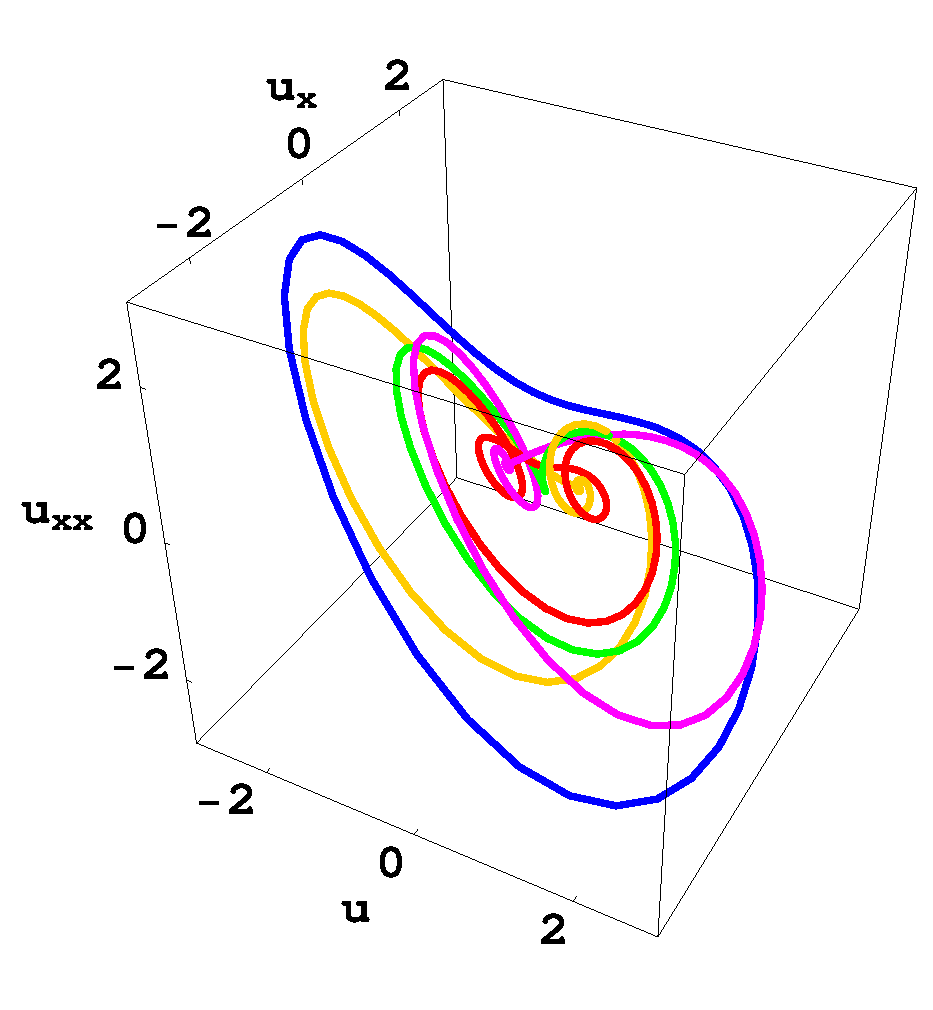
\includegraphics[width=0.4\textwidth]{figs/equilSpatial.eps}
\end{center}
\caption{
$(u,u_x,u_{xx})$ representation
of (blue) \EQV{1}, (red) \EQV{2},  (black) \EQV{3} \eqva,
 and (purple) \REQV{+}{1}, (orange) \REQV{-}{1} \reqva\ for
system size $L=22$. %, $N=64$ complex modes truncation.
        }
\end{figure}
%%%%%%%%%%%%%%%%%%%%%%%%%%%%%%%%%%%%%%%%%%%%%%%%%%%%%%%%%%%%%%%%%%

In a periodic box of size $L$
both \eqva\ and \reqva\ are  periodic solutions 
embedded in 3-$d$ space \refeq{eq:3dks}, 
conveniently represented as loops in 
$(u,v,w)$ space whose topology is controlled by
``\eqva\ of \eqva'' stable-unstable manifold structure of
\refeq{eqvEqvEigV}; see for example \reffig{f:eqvSpatial}.
In this representation the continuous translation symmetry
is automatic - a rotation in the $[0,L]$ periodic domain only
moves the points along the loop. For an \eqv\ the points
are stationary in time; for \reqv\ they move in time, but in
either case, the loop remains invariant.
So we do not have the problem that we encounter in the Fourier 
represenation, where from the frame of one of the \eqva\
the rest trace out circles under the action of continuous symmetry 
translations.


\subsection{When is an \eqv\ important? a bit of speculation} 

There are two kinds of roles
{\eqva} play:

{\em ``Hole'' in the natural measure}.
The more unstable eigendirections an \eqv\ has (for example, the
$u=$const \eqv~\EQV{0}), the more unlikely it is  that
an orbit will recur in its neighborhood.

{\em Unstable manifolds of the ``least unstable''{\eqva}}.
Empirically, asymptotic dynamics tends to spend
a large fraction of time in
neighborhoods of a few  {\eqva} with
only a few unstable eigendirections.


\subsection{Symmetries of \KSe}
% former \subsection{Scaling and symmetries}
% former symm.tex
% Predrag extracted from newton.tex         jul  3 2006

The  KS equation is
Galilean invariant: if $u(x,t)$ is a solution, then 
$v+u(x+2vt,t)$, with $v$ an arbitrary constant velocity, is also a solution. 
Without loss of generality, in our calculations we shall set 
the mean velocity of the  front to zero,
% \index{Galilean invariance}
% \index{invariance!Galilean}
\beq
\int dx \, u = 0
\,.
\ee{GalInv}
As  $\dot{a_0}=0$ in \refeq{expan}, 
$a_0$ is a conserved quantity, in our calculations
fixed to $a_0=0$ by the Galilean invariance condition \refeq{GalInv}.
The KS equation  \refeq{ks} is time translationally invariant,
and 
space translationally invariant
under the 1-$d$ Lie group of $O(2)$ rotations: if
$u(x,t)$ is a solution, then $u(x+d,t)$ is an equivalent
solution for any $-L/2 < d \leq L/2$.
The KS equation is also invariant under
reflection (``parity'' or ``inversion'') operation
\beq
\Refl u(x) = -u(-x)
\ee{KSparity}
and the shift symmetry operation 
\beq
\Shift u(x)=u(x+L/2)
\,. 
\ee{KSshift}
In the Fourier modes decomposition  this
symmetry corresponds to invariance under
\refeq{FModInvSymm}.
This shift symmetry is a particular case of the
above translational $O(2)$ invariance; more generally,
KS allows for solutions invariant under any rational shift by
$L/m$. Any \rpo\ with such rational shift is eventually periodic.
\Rpo s without a discrete symmetry have irrational shifts
$d$, and are not segments of a periodic solution.


Relations $\Refl^2=\Shift^2=1$
induce a linear decomposition of the space of solutions into 4 invariant
subspaces\rf{KNSks90} via projection operators
$\Refl_1=(\matId+\Refl)/2$,
$\Refl_2=(\matId-\Refl)/2$,
$\Shift_1=(\matId+\Shift)/2$, and
$\Shift_2=(\matId-\Shift)/2$. The nonlinear term $(u^2)_x$ in the KS equation
mixes these subspaces, leading,
according to \refref{KNSks90}, to four invariant subspaces
(labeled by the corresponding projection operators):
\begin{romannum} % SIAM itemize}

 \item[$R_1$:] The space of antisymmetric functions,
 \item[$S_1$:] The space of L/2 periodic functions,
 \item[$R_1 S_1$:] The intersection of the above two,
 \item[$L$:] The space of functions invariant under $x\mapsto L/2-x,\ u\mapsto -u$.
 
\end{romannum} %itemize}
%\ES{Using notation of \rf{KNSks90} here, not sure if it exists elsewere.}
The dynamics within the $R_1$ space of antisymmetric functions
was studied in \refref{Christiansen:97,Lan:Thesis,lanCvit06}.


\subsection{Antisymmetric subspace} 
\label{s:AntisymmSubsp}

Fix the  Poincar\'e section to be the hyperplane
$\Re a_1=0$. We integrate \refeq{expan} with the initial
 conditions
$\Re a_1=0$, and arbitrary values of the coordinates  $a_2, \ldots, a_N$, where
$N$ is the truncation order.  When $\Re a_1$ becomes
$0$ the next time,  the coordinates  $a_2, \ldots, a_N$ are mapped
into $(a_2', \ldots a_N')=P(a_2, \ldots, a_N)$, where $P$ is the  Poincar\'e
map. $P$ defines a mapping of a $N-1$ dimensional hyperplane into itself.
Under successive iterations of  $P$, any trajectory
approaches the attractor ${\cal A}$, which itself is an invariant
set under $P$.

A trajectory of
 (\ref{expan}) can cross the plane $a_1=0$ in two possible ways:
 either when
$\dot{a_1}>0$ (``up'' intersection)
or when  $\dot{a_1}<0$ (``down'' intersection),
 with the ``down'' and ``up'' crossings
alternating.
It then makes sense to define the  Poincar\'e map $P$ as a transition between,
say, ``up'' and ``up'' crossing.
With  Poincar\'e section defined as the ``up-up'' transition,
it is natural to define a ``down-up'' transition map $\Theta$. Since
$\Theta$ describes the transition from down to up (or up to down) state,
the map $\Theta^2$ describes the transition  up-down-up, that is
$\Theta^2=P$.

Now, with the help of the 
reflection $\mathbf{I}$ and shift symmetry $ \mathbf{S}$
operations
\refeq{KSparity},
\refeq{KSshift}
the  attractor ${\cal A}_{tot}$ can be
decomposed into four pieces:
 ${\cal A}_{tot}={\cal A} \cup S {\cal A}  \cup \Theta {\cal A}
  \cup \Theta S {\cal A} $. 

A decomposition
of the attractor into four disjoint sets
is usually not possible, since sometimes $ {\cal A}$ overlaps with
$\Theta S{\cal A} $ (in this case $\Theta  {\cal A}$ will also  overlap with
$S {\cal A} $).
In any case  the set $ {\cal A}$ can be taken as
the fundamental
domain of the Poincar{\'e} map, with $S  {\cal A} $,
$\Theta  {\cal A} $ and $\Theta S  {\cal A} $ its images under the
$S$ and $\Theta$ mappings.


% The Fourier coefficients $a_k$ are in general complex numbers.
% % of time $t$.  
% We can
% isolate the antisymmetric subspace of the system \refeq{ks-L} by
% considering the case of $a_k$ pure imaginary, $a_k= i a_k$, where
% $a_k$ are real, with the evolution equations
% \beq
% % \dot{a}_k=(k^2- k^4)a_k - k \sum_{m=-\infty}^{\infty} a_m a_{k-m}
% \dot{a}_k = (k/L)^2\left( 1 - (k/L)^2  \right)a_k 
%    - (k/L) \sum_{m=-\infty}^{+\infty} a_m a_{k-m}
% \,.
% \ee{expan-symm}

Since \KSe\ preserves
antisymmetric solutions, one can isolate the antisymmetric
subspace 
$u(x,t)=-u(-x,t)$, or in terms of Fourier coefficients,
$a_{-k}= - a_k$. 
For Fourier coefficients which respect the $x \to -x$ symmetry of
\KSe, see discussion in \refref{Christiansen:97},
and references therein.
In \refrefs{Christiansen:97,Lan:Thesis} 
this option was used to eliminate
the continuous translational symmetry.

In the antisymmetric subspace the translational 
invariance of the full system reduces
to the invariance under discrete
translation by half a spatial period $2\pi L$.
In the Fourier representation \refeq{expan}, 
this corresponds to invariance under 
\beq
a_{2m} \to a_{2m}\,, a_{2m+1} \to -a_{2m+1}
\,, m \in \mathbb{Z}
\,.
\ee{FModInvSymm} 
The antisymmetric condition amounts to imposing
$u(0,2\pi L)=0$ boundary condition, with
the size of the system reduced to
the $[0, \pi L]$ interval \ES{Greene and Kim show that steady states (non-traveling) 
have to be antisymmetric and our findings verify it. Thus when discussing equilibria this conversion is not
meaningfull.}.

In this paper we study the full \KS\ system invariant
under continuous translations. Due to the lack of self-adjointness
(non-normality) of the linearized \KS\ flow, 
the antisymmetric subspace
is unstable under small perturbations and generic solution of 
\KSe\ belongs to the full, periodic space. Nevertheless, some of
the \eqva\ and of the shortest periodic orbits lie in this subspace
and can play important role for the topology of the flow - examples
of such solutions will be discussed in \refsect{s:L22}.


\subsection{Stability of \eqva}
\label{s:StabEqui}
%%
% Predrag           5jun2005
% extracted from \Chapter{stability}{ 2apr2005}

If $u_\stagn(x)$ is an \eqv\ solution of \KSe,
the linear stability matrix
${\bf \Mvar}={\bf \Mvar}(a_\stagn)$
% , its matrix of its stability exponents
% in \refeq{die}
% local expansion rate
is constant in time,
and  
the {\jacobianM}
of the \eqv\ solution is
\[
 \jMps^t(a_\stagn) = e^{{\bf \Mvar} t}
    \,\qquad
 {\bf \Mvar}={\bf \Mvar}(a_\stagn)
\,.
\]
The matrix of variations
% \refeq{DerMatrix}
follows from \refeq{expan}
% \index{Kuramoto-Sivashinsky system}
\beq
{\Mvar}_{kj}(a) =\frac{\pde v_k(a)}{ \pde a_j  }
=((k/\tilde{L})^2- (k/\tilde{L})^4)\delta_{kj} - 2(k/\tilde{L}) a_{k-j}
\,.
\ee{expanMvar}
For the \KSe\ the constant solution $u(x,t)= E^{1/2}$ is an 
\eqv\ point of \refeq{ks} which we shall henceforth refer to as
\EQV{0}. For this ``laminar'' \eqv\ the {\stabmat}
is diagonal, and 
so is the {\jacobianM}
$
\jMps^t_{kj}(0) = \delta_{kj} e^{((k/\tilde{L})^2- (k/\tilde{L})^4)t}
\,.
$

As the system size $\tilde{L}$  is increased,
the ``flame front'' becomes increasingly unstable and turbulent,
the dynamics goes through a rich sequence of
bifurcations on which we shall not dwell here.
% studied e.g. in \refref{KNS90}. 
% , one quickly finds a
% myriad of unstable periodic solutions whose number
% grows exponentially with period.

The $|k|<??$ 
long wavelength perturbations of the flat-front {\eqv}
are linearly unstable, while all 
$|k|> ??$ short wavelength perturbations are strongly contractive.  
The high $k$ eigenvalues, corresponding to rapid variations of
the flame front, decay so fast that the corresponding eigendirections
are physically irrelevant.
% \index{Lyapunov exponent!{\eqv}}
To illustrate the rapid contraction in the non-leading eigendirections
we plot  in [MAYBE INCLUDE] % \reffig{f:eigenvalues}
the eigenvalues of the \eqv\ in the unstable regime,
for relatively small system size, % low viscosity $\nu$,
and compare them with the
stability eigenvalues of the least unstable cycle for the same 
system size.
The ``laminar'' \EQV{0}~\eqv\ is very unstable,
with many unstable eigendirections. 
However, for higher eigenvalues the rate of contraction
is so strong that higher eigendirections are numerically meaningless for 
either solution; even though the flow is infinite-dimensional, the attracting
set must be rather thin.


From \refeq{expan} we see that the origin $u(x,t) = 0$
has Fourier modes as the  linear
stability eigenvectors. 
When $|k| \in (0,\tilde{L})$, the corresponding Fourier modes are
unstable.
The most unstable modes has $|k|=\tilde{L}/\sqrt{2}$ 
and defines the scale of basic building
blocks of the spatiotemporal dynamics of the {\KSe} in large system size limit.
% as shown in \refsect{sec:KSnumer}. 


% \noindent
% Consider now the case of initial $a_k$ sufficiently small
% that the bilinear $ a_m a_{k-m}$ terms in \refeq{expan} can
% be neglected. Then we have a set of decoupled linear
% equations for $a_k$ whose solutions are exponentials, at most
% a finite number for  which
% $k^2 > \nu k^4$
% is growing with time, and infinitely many with
% $
% \nu k^4 > k^2
% $
% decaying in time.

% The growth of the unstable long wavelengths (low $|k|$) excites
% the short wavelengths
% through the nonlinear term in \refeq{expan}.  The excitations thus
% transferred are dissipated by the strongly damped short wavelengths,
% and a ``chaotic \eqv\'' can emerge. The very short
% wavelengths $|k| \gg 1 / \sqrt{\nu}$ remain small for all times,
% but the intermediate wavelengths of order $|k| \sim 1 / \sqrt{\nu}$
% play an important role in maintaining the dynamical {\eqv}.
% As the damping parameter decreases, the solutions increasingly take on
% % Burgers type
% shock front
% character poorly represented by the Fourier basis, and many
% higher harmonics may need to be kept
% % \rf{KNS90,GEP}
% in truncations of
% \refeq{expan}.
% 
% 
% Hence, while one may truncate the high modes in the expansion
% \refeq{expan}, care has to be exercised to ensure that no modes
% essential to the dynamics are chopped away. 
% 

Even though our starting point
\refeq{ks}
is an infinite-dimensional dynamical system, the asymptotic dynamics
unfolds on a finite-dimensional attracting manifold, and so we are back on
the familiar territory of 
%\refsect{SecDynFlows}:
the theory of a finite number of ODEs applies to this
infinite-dimensional PDE as well.

\subsection{Bifurcation structure of \KS}
\label{sec:KSlit}
% former KSlit.tex
%
% Vaggelis               jan 20 2007
% \subsection{\Eqva\ according to Greene and Kim}

In our study of the \eqva\ of
\KSe\ we follow the bifurcations analysis of
Kevrekidis, Nicolaenko and Scovel\rf{KNSks90} 
and
Greene and Kim\rf{ksgreene88}. What is new here is
a detailed exploration of the \eqva\ stable/unstable manifolds
for a specific system size $L = 22$, determination
of a large number of \rpo s, and a preliminary
exploration of the relation between the
observed spatiotemporal ``turbulent" patterns and
the \rpo s computed so far.


% What is the non-dimensional ``Rayleigh'' number for the
% \KS\ system? 
%  Scaling out the ``viscosity'' $\nu$ 
% \[ 
% x \to x \nu^{\frac{1}{2}}
% \,,\quad
% t \to t \nu
% \,,\quad
% u \to u \nu^{-\frac{1}{2}}
% \,,
% \]
% brings the \KSe\ \refeq{ks}
% to a non-dimensional form
% \beq
% u_t=(u^2)_x-u_{xx}- u_{xxxx}
% \,,\qquad 
%   x \in  [0,L\nu^{-\frac{1}{2}}] = [0,2\pi\tilde{L}]
% \,.
% \ee{ks-L}
% In this way the ``viscosity'' $\nu$
% and the system size $L$ are trade in for a single
% dimensionless system size parameter
% \beq
%   \tilde{L}={L}/{(2 \pi \sqrt{\nu})}
% % \tilde{L}=\frac{L}{2 \pi \sqrt{\nu}}
% % \,,
% \ee{tildeL}
% which plays the role of a ``Reynolds number''
% for the \KS\ system.

In the literature \refeq{ks} is sometimes written as
\beq
    u_t=(u^2)_x-u_{xx}- \nu \, u_{xxxx}
    \,,\qquad   x \in [0,L]
    \,,
\ee{ksVisc}
or in any number of other variants, all equivalent.
Here we use
$L$ as the system parameter, with the ``hyper-viscosity" $\nu$ fixed to $1$.
Other authors is vary  $\nu$, with $L$ fixed to either $1$ or $2\pi$.
To minimize confusion,
in what follows we shall state results of all 
calculations either in units of the dimensionless system size $\tildeL$,
or the systems size $L = 2 \pi \tildeL$. The parameter $\alpha$
of \refrefs{KNSks90,ksgreene88} is in this convention is
$\tildeL=\sqrt{\alpha/4}$.


For small $\tildeL$ the only \eqv\ of the system is the constant solution $y(x,t)=0$,
globally attracting 
for $\tildeL<1$. At $\tildeL=N$, $N=1,2,3, \dots$, 
the $N$th harmonic becomes unstable and the constant solution
bifurcates to the antisymmetric ``$N$-cell'' states\rf{ksgreene88}. 
These states contain only the multiples of the $N$th
harmonic, {\ie}, only the components $a_N,a_{2N},...$ in our notation.
Greene and Kim show that symmetric solutions are \eqva, not \reqva. 
% At point $A$ in \reffig{fig:GreeneKim}
At point $A$ in \reffig{fig:ksBifDiag}
the $1$-cell state loses stability
and bifurcates to a stable, 
asymmetric \reqv, which later on becomes unstable through a Hopf bifurcation. 

At $\tildeL=2$ the system has become large enough 
that a $2$-cell \eqv\ appears. 
% At point $B$ in \reffig{fig:GreeneKim}
At point $B$ in \reffig{fig:ksBifDiag}
the $1$-cell branch merges to the $2$-cell branch. 
In general each $N$-cell branch merges to the corresponding $2N$-cell branch.

% At point $C$ in \reffig{fig:GreeneKim}
At point $C$ in \reffig{fig:ksBifDiag}
the $2$-cell state bifurcates to a type of 
\eqv\ solution
found by La Quey, Mahajan, Rutherford and Tang\rf{laquey74} and generalized by Greene and Kim who refer to them as GLMRT \eqva. GLMRT solutions are symmetric 
($u(x)$ is antisymmetric)
and can be roughly described as long-wave distorted $N$-cell states.

% The last type of solution identified in \refref{ksgreene88} appears at point $F$ 
% in \reffig{fig:GreeneKim} and is called a
% ``giant" state because its amplitude grows as the system size increases.

According to the bifurcation diagram 
% \reffig{fig:GreeneKim}, 
\reffig{fig:ksBifDiag}, 
at the point that corresponds to system size $\tildeL=22/2\pi \simeq 3.5$
studied here,
the {\eqva} we expect are the $2$- and $3$-cell states \EQV{2} and \EQV{3},
the GLMRT state that bifurcates from a $3$-cell state at point $I$ (\EQV{1}),
the pair of \reqva\ that belong to the branches starting at points $A$ (\REQV{\pm}{1}),
and the $M$ branch  \reqva\ \REQV{\pm}{2}.

%%%%%%%%%%%%%%%%%%%%%%%%%%%%%%%%%%%%%%%%%%%%%%%%%%%%%%%%%%%%%%%%
\begin{figure}[t]
\begin{center} 
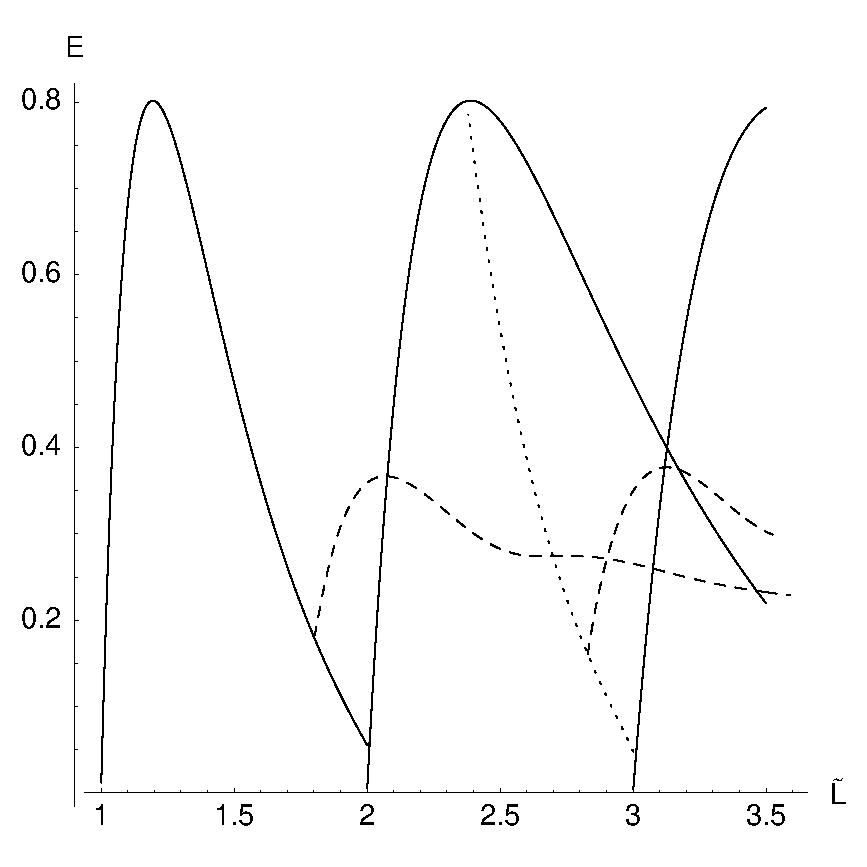
\includegraphics[width=0.5\textwidth]{figs/ksBifDiag.eps}
\end{center}
\caption{
The ``energy'' \refeq{ksEnergy}  of \eqva\
plotted as a function of the system size
$\tildeL$ (recomputed following \refref{ksgreene88}), tracked to
$\tildeL \approx 3.5$ studied here.
Solid curves denote $N$-cell solutions,
dotted curves GLMRT, the dash-dotted curve the
giant states, and dashed curves the propagating solutions.
Open circles indicate Hopf bifurcations. 
The color of a branch indicates the number of unstable
eigenvalues: (red) 2 unstable eigenvalues, (blue) 1
unstable eigenvalue, (green) stable. 
\ESedit{
ES: Shown is the 2c to GLMRT bifurcation and the GLMRT to \REQV{\pm}{2} bifurcation, 
points C and M in \rf{ksgreene88} respectively.
       } 
        }
\label{fig:ksBifDiag}
\end{figure}
%%%%%%%%%%%%%%%%%%%%%%%%%%%%%%%%%%%%%%%%%%%%%%%%%%%%%%%%%%%%%%%%%%

        \PublicPrivate{%
        }{% switch to Private:

\subsection{Back in the saddle again}

Kevrekidis, Nicolaenko and Scovel~\rf{KNSks90} study \KSe\ 
\eqva, their 
bifurcations and the role of symmetry in the existence of 
structurally stable (relative) homoclinic and heteroclinic connections 
between unstable saddles. The form  of the equation they use is
essentially that of Greene and Kim but with bifurcation parameter 
connected to our by $\alpha=4\tilde{L}^2$.


They prove that the bifurcation of the trivial state $y=0$ to an $N$-cell state is a pitchfork. 
They observe that when the $1$-cell state losses stability at point $A$ the
eigenvector corresponding to the zero eigenvalue of the stability matrix aligns itself with the direction of uniform translation of the
system which, due to the translational invariance of \KSe\, also corresponds to a zero eigenvalue. Thus the algebraic multiplicity of the zero eigenvalue is $2$ while its geometric multiplicity is $1$. Using this fact and a local, $O(2)$-equivariant, approximation to the center manifold they prove that this type of bifurcation creates traveling waves.

In typical numerical simulations  a trajectory initiated along the (single) unstable eigendirection of a
fixed point $y$ of the $2$-cell branch would eventually become attracted to the $L/4$-translated equilibrium $y'$. 
Those (relative) homoclinic connections 
\ES{In \refref{KNSks90} the characterization homoclinic connection is used. Here
we prefer (to invent?) the term relative homoclinic to emphasize the fact that the fixed points are symmetry related.} although structurally unstable in most dynamical systems, were found to be persistent in KSe with the afore-mentioned behaviour observed in the range  
from $\tilde{L}\simeq 2.009$ up to $\tilde{L}\simeq 2.375$  where the $2$-cell state becomes stable. The existance and
robustness of the saddle connection was explained as follows\ES{The following may not make perfect sense without reading the paper, especially the
notation. I've start re-writing \KS\ symmetries section to incorporate information about the invariant subspaces which hopefully will explain it but
my progress is very slow.}:  The unstable manifold of $y$ lies on an invariant subspace $L$ of
\KS\ flow, which is the fixed set of the isotropy subgroup of $O(2)$ defined by reflection with respect to imaginary axis. The action of the generator of $D(4)$ (which sents y to y') on $L$ is to send it to the invariant subspace $R_{1}$ which is the fixed set of $Z(2)$ defined by complex
conjugation. The converse is also true, i.e. the action of $D(4)$ sents $R_{1}$ to $L$. Thus the unstable eigendirection of $y$, lying on $L$, is sent on $R_{1}$ for the $L/4$-shifted point $y'$. The two invariant subspaces $L$ and $R_{1}$ are orthogonal and thus the point $y'$ has only stable eigendirections on $L$ and appears as a sink on that subspace. This explains why the (relative) homoclinic connections are structurally stable in \KSe.

In the range $\tilde{L}=2.00$ when the $2$-cell branch comes to existance with two unstable eigendirections, up to $\tilde{L} \simeq 2.009$ when it
merges to the $1$-cell branch and losses one of its unstable eigendirections, a heteroclinic loop exists that connects $2$-cell to $1$-cell solutions.
The analysis is similar to the previous case.

An important remark in \refref{KNSks90} is that the exact saddle connections were observed using a numerical integrator based on an explicit Galerkin spectral discretezation of \KSe, irrespective of how close to the equilibrium along the unstable manifold we start. On the contrary, when an FFT-based integrator was used, trajectories with initial condition along the unstable direction of $y$ would approach the homoclinic connection but fly away along the direction of the unstable manifold of $y'$ and follow an approximate (relative) homoclinic loop. This is attributed to the Galerkin truncation respecting the symmetries and possesing the same subspaces as the original equation restricted to the first $n$ modes \ES{We observe the second kind of behavour and we both use an FFT based integrator. I plan to quikly write a Galerkin integrator and check to see if we get an exact connection.}.

        } %end \PublicPrivate{%

